\documentclass[11pt, a4paper]{article}

\usepackage{graphicx}
\usepackage[english]{babel}
\usepackage[utf8x]{inputenc}
\usepackage{amsmath}
\usepackage[a4paper,top=3cm,bottom=2cm,left=2cm,right=2cm,marginparwidth=1.75cm]{geometry}
\usepackage{amssymb}

\graphicspath{ {./images} }
\newcommand*{\qed}{\hfill\ensuremath{\quad\square}}%
\newcommand*{\rad}{\ensuremath{\,\text{rad}}}
\newcommand*{\R}{\ensuremath{\mathbb{R}}}

\makeatletter
\renewcommand*\env@matrix[1][*\c@MaxMatrixCols c]{%
  \hskip -\arraycolsep
  \let\@ifnextchar\new@ifnextchar
  \array{#1}}
\makeatother

\newtheorem{theorem}{Theorem}

%------------------------------------------------
%Templates for images and figures
% \begin{figure}[h]
%   \centering
%   \subfloat[caption 1]{{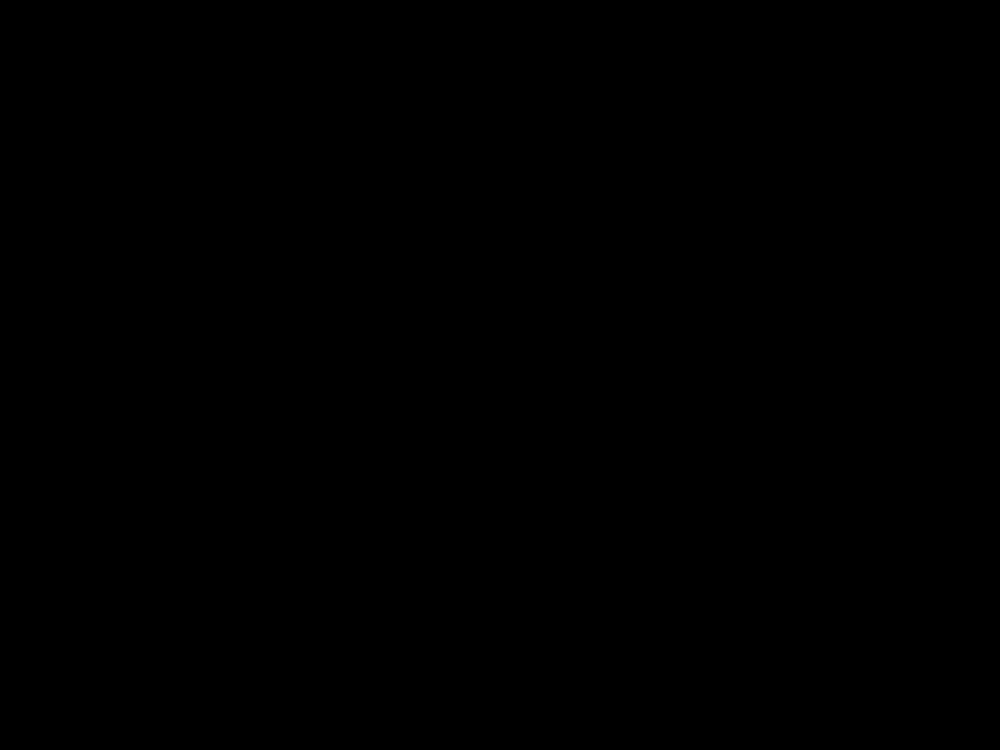
\includegraphics[width=30mm]{images/placeholder.png}}}%
%   \qquad
%   \subfloat[caption 2]{{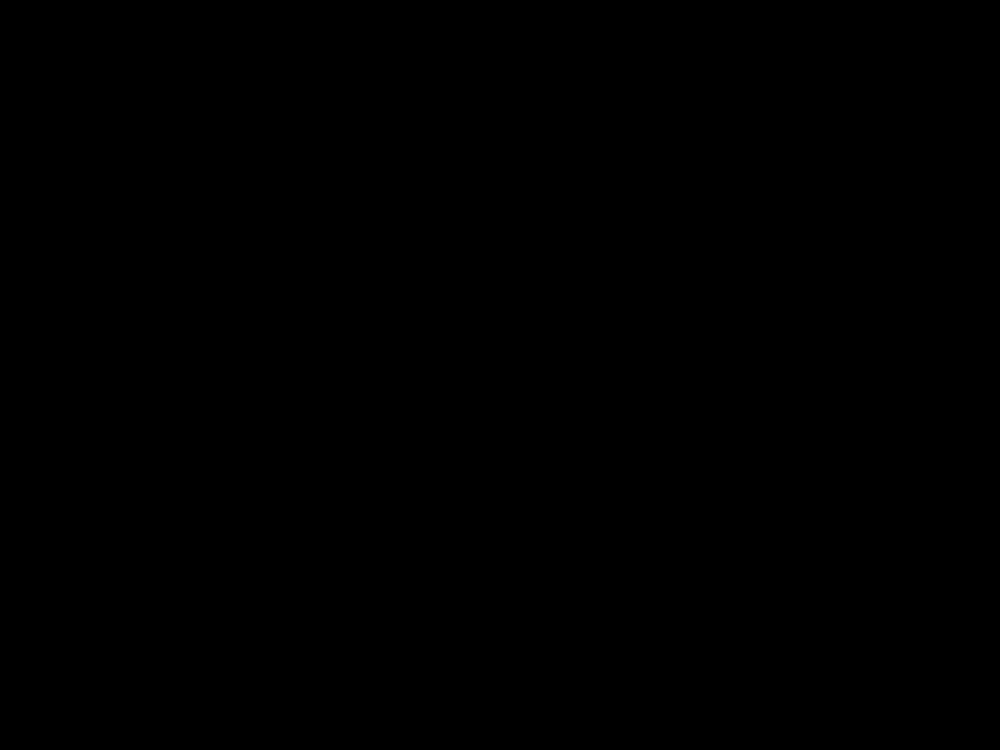
\includegraphics[width=30mm]{images/placeholder.png}}}%
%   \caption{Description}
% \end{figure}

% \begin{figure}[h]
%   \centerline{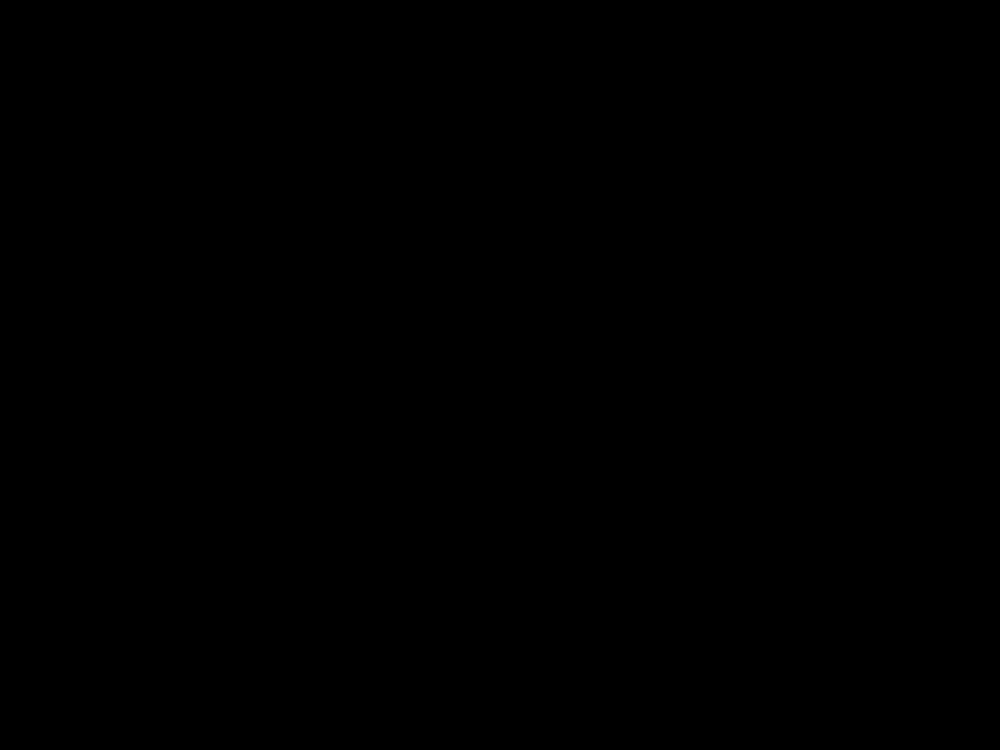
\includegraphics[width=50mm]{images/placeholder.png}}
%   \caption{Description}
% \end{figure}
%-----------------------------------------------

\begin{document}
\section{Impulse and momentum of rigid bodies}
\subsection{The cross product}
Since the cross product is very important for rigid body dynamics a quick definition will be given here. The cross product has been briefly covered in previous lecture notes before. The cross product between 2 vectors is defined as follows:
\begin{gather}
  \vec{a} \times \vec{b} = ||\vec{a}||\,||\vec{b}||\sin(\theta)\cdot \vec{n}
\end{gather}
$\theta$ is the angle between the vectors $\vec{a}$ and $\vec{b}$, and $\vec{n} \in W^\perp$ where the subspace $W$ is the span of vectors $\vec{a}$ and $\vec{b}$. This is the more formal definition of the cross-product but the more practical way of doing computations is done with the following expression:
\begin{align}
  \vec{a} \times \vec{b} =
  \begin{vmatrix}
    \hat{i} & \hat{j} & \hat{k}\\
        a_1 & a_2     & a_3\\
        b_1 & b_2     & b_3\\
  \end{vmatrix}
  &=
  \begin{vmatrix}
    a_2 & a_3\\
    b_2 & b_3\\
  \end{vmatrix}
  \hat{i} -
  \begin{vmatrix}
    a_1 & a_3\\
    b_1 & b_3\\
  \end{vmatrix}
  \hat{j} +
  \begin{vmatrix}
    a_1 & a_2\\
    b_1 & b_2\\
  \end{vmatrix}
  \hat{k}\\
  &= (a_2b_3 - a_3b_2)\hat{i} - (a_1b_3 - a_3b_1)\hat{j} + (a_1b_2 - a_2b_1)\hat{k}
\end{align}

\subsection{Angular momentum of rotating rigid bodies}
Since the theory behind rotating point masses and rigid bodies is almost the exact same this lecture will only really cover the additional new material. Lecture notes for lecture 08 contain more indepth notes about conservtion of angular momentum so look at those if this is still difficult.\\
\\
The angular momentum of a rotating rigid-body is given by:
\begin{equation}
  H_G = I_G\omega
\end{equation}
If it is desired to compute the angular momentum around a point $A$ which is not in fact the centroid the expression becomes:
\begin{equation}
  \vec{H}_A = I_G\vec{\omega} + \vec{r}_{G/A} \times m\vec{v}_G
\end{equation}
Which is nothing but the angular momentum around the centroid with the added linear momentum of point $A$ relative to the centroid.
\begin{equation}
  \int_{t_1}^{t_2} M_A\,dt = \vec{r}_2 \times m\vec{v}_2 - \vec{r}_1 \times m\vec{v}_1 = \vec{H}_{A2} - \vec{H}_{A1} 
\end{equation}
if $\int_{t_1}^{t_2} M_A\,dt = 0$ angular momentum is coserved.

\end{document}